%%%%%%%%%%%%%%%%%%%%%%%%%%%%%%%%%%%%%%%%%
% Beamer Presentation
% LaTeX Template
% Version 1.0 (10/11/12)
%
% This template has been downloaded from:
% http://www.LaTeXTemplates.com
%
% License:
% CC BY-NC-SA 3.0 (http://creativecommons.org/licenses/by-nc-sa/3.0/)
%
%%%%%%%%%%%%%%%%%%%%%%%%%%%%%%%%%%%%%%%%%

%----------------------------------------------------------------------------------------
%	PACKAGES AND THEMES
%----------------------------------------------------------------------------------------

\documentclass{beamer}

\mode<presentation> {

% The Beamer class comes with a number of default slide themes
% which change the colors and layouts of slides. Below this is a list
% of all the themes, uncomment each in turn to see what they look like.

%\usetheme{default}
%\usetheme{AnnArbor}
%\usetheme{Antibes}
%\usetheme{Bergen}
%\usetheme{Berkeley}
%\usetheme{Berlin}
%\usetheme{Boadilla}
%\usetheme{CambridgeUS}
%\usetheme{Copenhagen}
%\usetheme{Darmstadt}
%\usetheme{Dresden}
%\usetheme{Frankfurt}
%\usetheme{Goettingen}
%\usetheme{Hannover}
%\usetheme{Ilmenau}
%\usetheme{JuanLesPins}
%\usetheme{Luebeck}
\usetheme{Madrid}
%\usetheme{Malmoe}
%\usetheme{Marburg}
%\usetheme{Montpellier}
%\usetheme{PaloAlto}
%\usetheme{Pittsburgh}
%\usetheme{Rochester}
%\usetheme{Singapore}
%\usetheme{Szeged}
%\usetheme{Warsaw}

% As well as themes, the Beamer class has a number of color themes
% for any slide theme. Uncomment each of these in turn to see how it
% changes the colors of your current slide theme.

%\usecolortheme{albatross}
%\usecolortheme{beaver}
%\usecolortheme{beetle}
%\usecolortheme{crane}
%\usecolortheme{dolphin}
%\usecolortheme{dove}
%\usecolortheme{fly}
%\usecolortheme{lily}
%\usecolortheme{orchid}
%\usecolortheme{rose}
%\usecolortheme{seagull}
%\usecolortheme{seahorse}
%\usecolortheme{whale}
%\usecolortheme{wolverine}

%\setbeamertemplate{footline} % To remove the footer line in all slides uncomment this line
%\setbeamertemplate{footline}[page number] % To replace the footer line in all slides with a simple slide count uncomment this line

\setbeamertemplate{navigation symbols}{} % To remove the navigation symbols from the bottom of all slides uncomment this line
%\setbeamertemplate{itemize items}[triangle]
}

\usepackage{graphicx} % Allows including images
\usepackage{booktabs} % Allows the use of \toprule, \midrule and \bottomrule in tables

\usepackage{longtable}
\usepackage{multirow}
\usepackage{dcolumn}
\usepackage{bigstrut}
\usepackage{dcolumn}
\newcolumntype{d}[1]{D{.}{.}{#1}}
%\usepackage[group-separator={.}]{siunitx}
\usepackage{xcolor,colortbl}
\definecolor{Gray}{gray}{0.85}
\usepackage{siunitx}
\usepackage{colortbl}
%\usepackage{arydshln}
\usepackage{adjustbox} % to use adjustbox command - change size of the table

\usepackage{rotating}
\usepackage{epstopdf}

%\usepackage[longnamesfirst,semicolon]{natbib}
%\bibliographystyle{agsm}
%\usepackage[citestyle=authoryear]{biblatex}
\usepackage[backend=bibtex,style=authoryear, natbib]{biblatex}
\bibliography{Surprise_Lit.bib}

%----------------------------------------------------------------------------------------
%	TITLE PAGE
%----------------------------------------------------------------------------------------

\title[Surprise in Short Interest]{ \textbf{Surprise in Short Interest}}  % The short title appears at the bottom of every slide, the full title is only on the title page


\author[Pavel Lesnevski]{Pavel Lesnevski\inst{1}   \and Esad Smajlbegovic\inst{2}}
\institute[University of Mannheim]{          \inst{1} University of Mannheim \and
                     \inst{2} Erasmus University Rotterdam}

\date{March 17, 2017} % Date, can be changed to a custom date

\begin{document}

\begin{frame}
\titlepage % Print the title page as the first slide
\end{frame}

%\begin{frame}
%\frametitle{Overview} % Table of contents slide, comment this block out to remove it
%\tableofcontents % Throughout your presentation, if you choose to use \section{} and \subsection{} commands, these will automatically be printed on this slide as an overview of your presentation
%\end{frame}

%----------------------------------------------------------------------------------------
%	PRESENTATION SLIDES
%----------------------------------------------------------------------------------------
%============================================================================

\section{Introduction}
\begin{frame}
	\frametitle{Motivation}
	%\framesubtitle{Bullet points}
	
	\begin{itemize}
		\item Short-selling activity predicts stock returns\\ 
		\begin{scriptsize}
		\citep[e.g.,][]{desai_investigation_2002,boehmer_which_2008,diether_short-sale_2009,akbas_short_2013,rapach_short_2016}	
		\end{scriptsize}
		
		\item Main measure - number of shares shorted relative to shares outstanding (short interest ratio).
		
		\item Different interpretations of this predictability:
		\begin{itemize}
			\item Binding short sale constraints result in overpricing 					\begin{scriptsize}\\
				\citep[e.g.,][]{miller_risk_1977, asquith_short_2005} 
			\end{scriptsize}	
			\vspace*{0.1cm}
			\item Short-selling is risky and costly 
			\begin{scriptsize}\\
				\citep[e.g.,][]{drechsler_shorting_2016,hong_days_2016, engelberg_short_2016} 
			\end{scriptsize}
			\item Persistent mispricing  \\
			{\scriptsize \citep[e.g.,][]{boehmer_good_2010}}
		\end{itemize}
		
		\item Little evidence on predictive ability for changes in short interest \\
		 {\scriptsize \citep{boehmer_good_2010}}
		 	
	\end{itemize}
\end{frame}
%============================================================================
\begin{frame}
	\frametitle{This paper}
	%\framesubtitle{Bullet points}
	\begin{itemize}
		\item ...proposes a new measure of informed short selling - \textbf{surprise in short interest} - that
		\begin{itemize}
			\item reflects changes in short-sellers' positions
			\item associated with strong price drift around short interest announcement
			\item predicts stock's future fundamental news
			\item not explained by short-sale constraints, common mispricing and risk factors	
			\item related to other proxies for limits to arbitrage
		\end{itemize} 
\item[$\Rightarrow$]   Mispricing-based interpretation of return predictability.
	\end{itemize}
\end{frame}
%============================================================================

\begin{frame}
		\frametitle{Surprise in Short Interest}
\begin{figure}[htbp]
	 \centering
	 \vspace*{-0.3cm}
	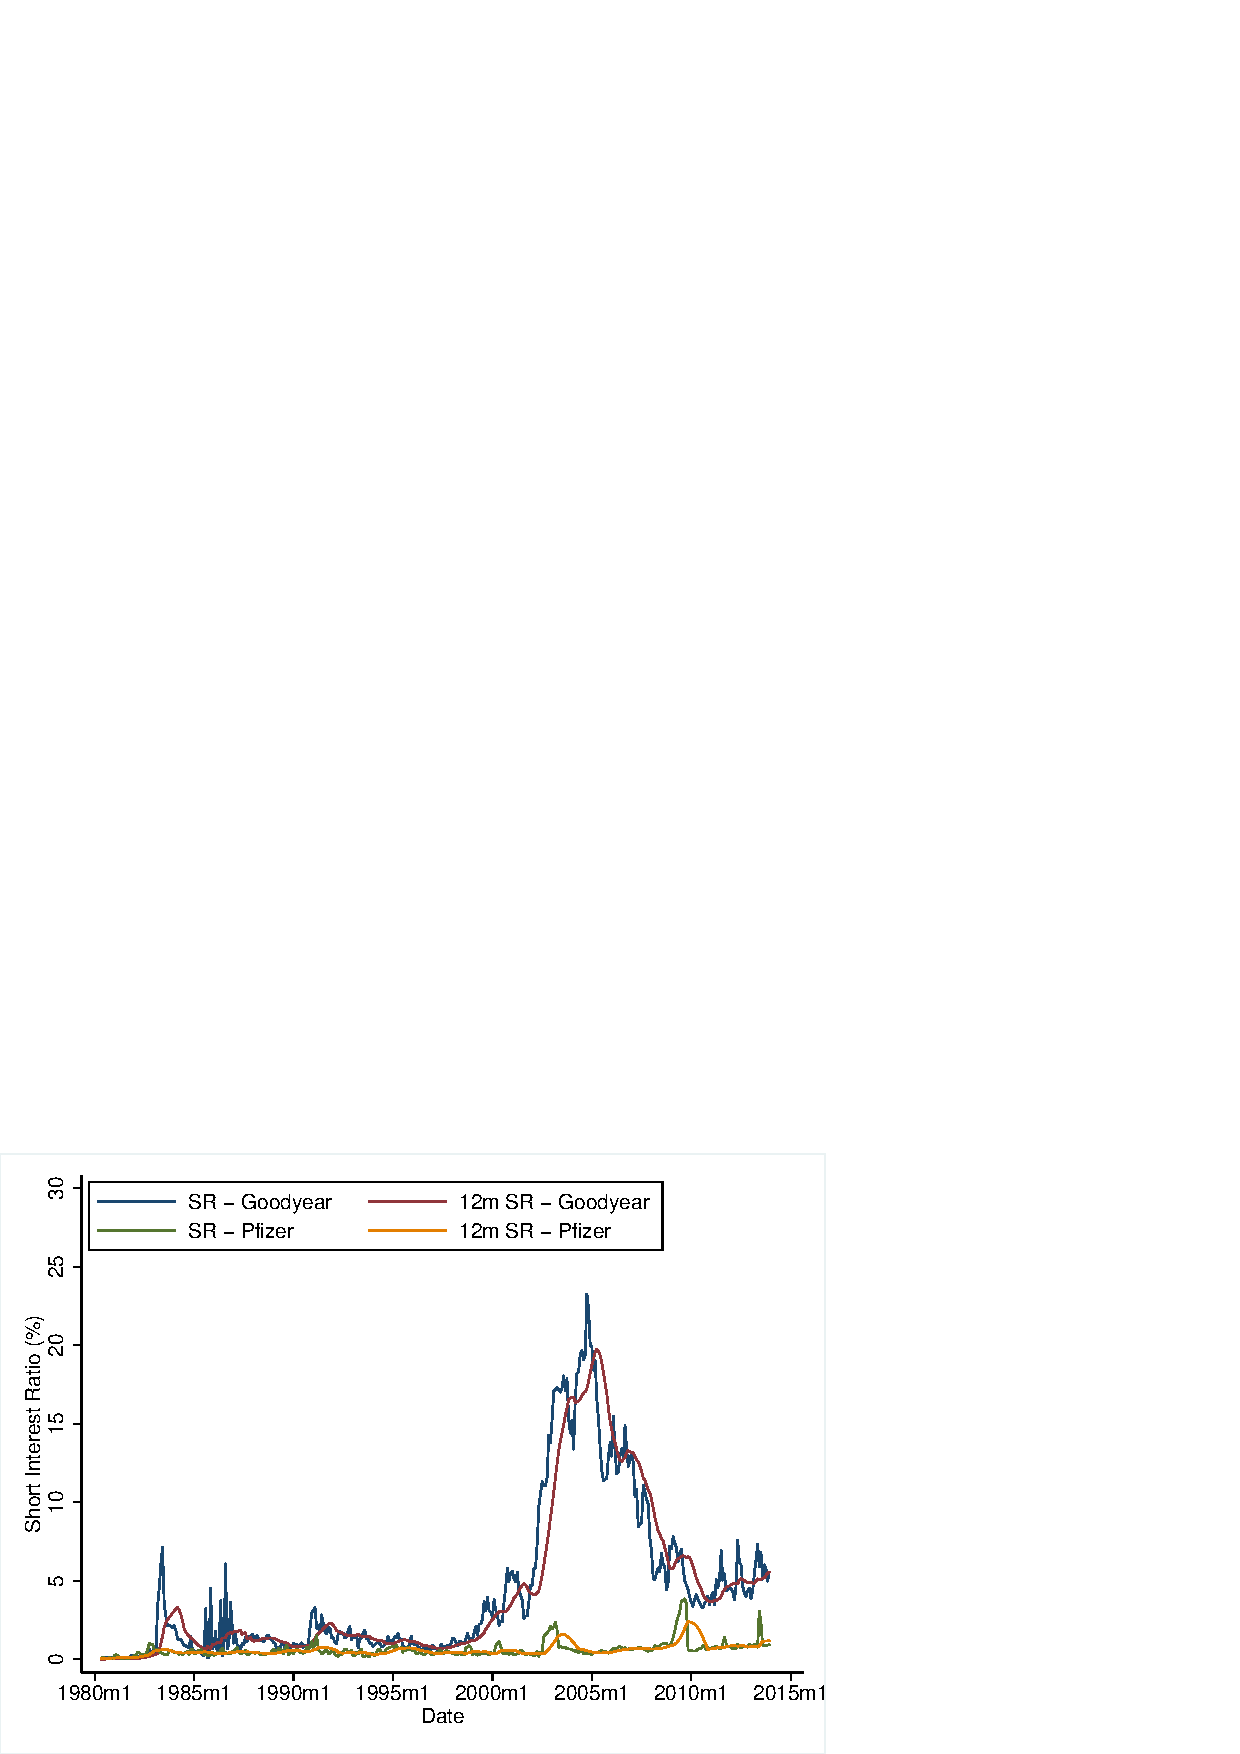
\includegraphics[scale=0.6,trim=4 4 4 4,clip]{figures/intro_graph.pdf} 
	% \caption[]{\textbf{\\Cumulative Logarithmic Raw Returns}\\
    % \footnotesize{Plotted are the monthly cumulative sum of log raw returns for equal-weighted and value-weighted $SUSIR$ long-short strategy over the period from March 1980 to December 2013.}}
	\label{tab:cumLS}%
\end{figure}
\vspace*{-0.4cm}
	\begin{itemize}
\item High time-series persistence of short interest within stocks
\item Difference in the volatility of short interest across stocks

\item[$\Rightarrow$] Non-informative short-selling contaminates informativeness of short interest ratio
	\end{itemize}
\end{frame}

%============================================================================

\begin{frame}
		\frametitle{Surprise in Short Interest}
\begin{itemize}
\item \textbf{Suprise in short interest} defined as the standardized unexpected short interest ratio (SUSIR)
\end{itemize}	
\begin{equation} \nonumber
SUSIR_{i,t} = \frac{SR_{t} - \overline{SR}_{t-1,t-12}}{\sigma^{SR}_{t-1,t-12}},
\label{eq:susir}
\end{equation} 
\begin{enumerate}
	\item Extract unexpected component of short interest ratio by subtracting 12-months moving mean
	\item Relate this component to the variation of the short interest ratio
\end{enumerate}

\end{frame}
%============================================================================

\begin{frame}
		\frametitle{Surprise in Short Interest - Announcement}
		\vspace*{-0.3cm}
\begin{figure}[htbp]
	 \centering
	\includegraphics[scale=0.39]{figures/Event_study_High_dec_susir.pdf} 
	% \caption[]{\textbf{\\Cumulative Logarithmic Raw Returns}\\
    % \footnotesize{Plotted are the monthly cumulative sum of log raw returns for equal-weighted and value-weighted $SUSIR$ long-short strategy over the period from March 1980 to December 2013.}}
\end{figure}
\vspace*{-0.9cm}
\begin{figure}[htbp]
	 \centering
	\includegraphics[scale=0.39]{figures/Event_study_Low_dec_susir.pdf} \\
	% \caption[]{\textbf{\\Cumulative Logarithmic Raw Returns}\\
    % \footnotesize{Plotted are the monthly cumulative sum of log raw returns for equal-weighted and value-weighted $SUSIR$ long-short strategy over the period from March 1980 to December 2013.}}
%This figure displays the cumulative average abnormal returns (CAARs) of two portfolios based on the surprise in short interest. The benchmark is the market return and the time window is 10 days before and 30 days after the NYSE's short interest dissemination day. Figure~\ref{Event_study_High_dec_susir} plots the CAAR for stocks with the highest 30\% of surprises in short interest at each event day, whereas Figure~\ref{Event_study_Low_dec_susir} plots the CAAR for stocks with the lowest 30\% of surprises in short interest at each event day. The dashed lines represent the upper and lower 90\% confidence intervals. The sample starts in January 1995 and contains stocks traded on the NYSE.
\vspace*{-0.2cm}
\scriptsize{Top 30\% (upper graph) and bottom 30\% (lower graph) surprises, NYSE stocks over 1995-2013}
\end{figure}
\end{frame}
%============================================================================


\section{Data}
\begin{frame}
	\frametitle{Data sources}
\begin{itemize}
\item Sample period: March 1980 -- December 2013
\item Sample selection:
\begin{itemize}
\item stocks with share code 10 and 11
\item AMEX, NYSE, NASDAQ traded stocks
\item Price greater than USD 5 and market cap greater than the 5th percentile of the NYSE distribution
\end{itemize}
\ \\
\ \\
\item Equity market data on stock level: CRSP
\item Accounting data: Compustat annual file
\item Short interest: Compustat supplementary short interest file
\item Institutional ownership: TR 13F Filings
\item Mispricing score and risk factors: Authors' website
\ \\
\ \\
\item Variables are standardized with zero mean and unit standard deviation
\end{itemize}
\end{frame}

%============================================================================

	\begin{frame}
		\frametitle{Predictability of Stock Returns}
				\framesubtitle{Fama-MacBeth Regression Approach}	

\begin{table}[htbp]
  \centering
  \vspace*{-0.2cm}
 % \footnotesize
 %    \captionsetup{width=\textheight}
 % \caption[]{\textbf{\\ Fama-MacBeth Regression of Stock Returns on $SUSIR$  }\\
%     \footnotesize{This table reports results of the Fama-MacBeth regression of raw monthly stock returns on $SUSIR$ measure and other stock characteristics. All explanatory variables are normalized to have mean equal to zero and standard deviation equal to one. Additional control variables are market beta, log size, log book-to-market ratio, momentum and short-term reversal. The t-statistics are \cite{newey_hypothesis_1987} adjusted. ***, ** and * indicate significance at 1\%, 5\% and 10\% levels, correspondingly.
  %      }}
		%\begin{adjustbox}{width=\linewidth , totalheight= \textheight, keepaspectratio}
	  \resizebox{0.65\textwidth}{!}{	 	
	 
    \begin{tabular}{lccccc}
    \toprule
          & (1)   & (2)   & (3)   & (4)   & (5) \\
            & $Ret_{i,t}$   & $Ret_{i,t}$   & $Ret_{i,t}$   & $Ret_{i,t}$   & $Ret_{i,t}$ \\
          \midrule
\rowcolor[rgb]{ .769,  .843,  .608}       $SUSIR$ & -0.114*** & -0.0852*** & -0.0928*** & -0.0812*** & -0.0766*** \\
\rowcolor[rgb]{ .769,  .843,  .608}             & (-5.73) & (-4.55) & (-4.60) & (-3.97) & (-4.04) \\
    $SR$  &       & -0.404*** &       &       & 0.168* \\
          &       & (-4.77) &       &       & (1.70) \\
    $DTC$ &       &       & -0.169*** &       & -0.0998** \\
          &       &       & (-4.98) &       & (-2.28) \\
    $SR_{IO}$ &       &       &       & -0.234*** & -0.168*** \\
          &       &       &       & (-6.55) & (-3.14) \\
    $INV$ &       &       &       &       & 0.0280 \\
          &       &       &       &       & (0.85) \\
    $ROA$ &       &       &       &       & -0.0673 \\
          &       &       &       &       & (-1.20) \\
    $MISP$ &       &       &       &       & -0.222*** \\
          &       &       &       &       & (-4.75) \\
    $IVOLA$ &       &       &       &       & -0.318*** \\
          &       &       &       &       & (-4.95) \\
          \midrule
	$Controls$ & Yes & Yes &Yes & Yes &Yes \\    
    $N$   & 577088 & 577088 & 577056 & 475372 & 470396 \\
    $R^2$ & 0.058 & 0.062 & 0.061 & 0.061 & 0.084 \\
    \bottomrule
    \end{tabular}%
	}
\end{table}
\begin{itemize}
\item[$\rightarrow$] Robust to existing short-interest and mispricing-based predictors
\end{itemize}

\end{frame}
%============================================================================
\section{Results}	
	\begin{frame}
		\frametitle{Predictability of Stock Returns}	
		\framesubtitle{Portfolio Sorts}	
		
% Table generated by Excel2LaTeX from sheet 'portfolio_sorts_combined'
\begin{table}[htbp]
  \centering
%  \caption{Add caption}
	  \resizebox{0.8\textwidth}{!}{	 	 
    \begin{tabular}{lccccccc}
    \toprule
          & \multicolumn{3}{c}{Equal-Weighted Portfolio} &       & \multicolumn{3}{c}{ Value-Weighted Portfolio} \\
\cmidrule{2-4}\cmidrule{6-8}    Decile & RawRet & CAPM  & C4    &       & RawRet & CAPM  & C4 \\
    \midrule
    1 (Long) & 1.002 & 0.359 & 0.239 &       & 0.862 & 0.278 & 0.220 \\
    2     & 0.936 & 0.290 & 0.121 &       & 0.830 & 0.249 & 0.249 \\
    3     & 0.875 & 0.233 & 0.079 &       & 0.640 & 0.048 & -0.051 \\
    4     & 0.849 & 0.215 & 0.032 &       & 0.636 & 0.019 & -0.045 \\
    5     & 0.786 & 0.151 & -0.018 &       & 0.598 & 0.004 & -0.017 \\
    6     & 0.790 & 0.151 & -0.006 &       & 0.729 & 0.124 & 0.104 \\
    7     & 0.659 & -0.002 & -0.172 &       & 0.604 & 0.040 & -0.040 \\
    8     & 0.634 & -0.031 & -0.208 &       & 0.356 & -0.229 & -0.339 \\
    9     & 0.517 & -0.149 & -0.276 &       & 0.580 & -0.016 & -0.054 \\
    10 (Short) & 0.572 & -0.098 & -0.250 &       & 0.515 & -0.073 & -0.147 \\
    \midrule

\rowcolor[rgb]{ .769,  .843,  .608}     1-10  & 0.430 & 0.458 & 0.489 &       & 0.347 & 0.350 & 0.368 \\
\rowcolor[rgb]{ .769,  .843,  .608}            & (5.287) & (5.498) & (5.703) &       & (3.304) & (3.012) & (3.132) \\
   L 30\% - H 30\% & 0.363 & 0.387 & 0.391 &       & 0.293 & 0.297 & 0.313 \\
         & (6.633) & (6.892) & (6.526) &       & (3.582) & (3.186) & (3.538) \\
    \bottomrule
    \end{tabular}%
    }
  \label{tab:addlabel}%
\end{table}%
\vspace*{-0.3cm}
\begin{itemize}
\item[$\rightarrow$] Strong for EW and VW portfolios and robust to various factor models
\end{itemize}
\end{frame}

%============================================================================
	
\begin{frame}

\frametitle{Performance Over Time}

\begin{figure}[htbp]
\centering
	\includegraphics[scale=0.7,trim=4 4 4 4,clip]{figures/cumLS_susir_both_11.pdf} 
	\label{tab:cumLS}%
\end{figure}
\begin{itemize}
\vspace*{-0.7cm}
\item[$\rightarrow$] Stable performance over sample period
\end{itemize}
\end{frame}
%============================================================================


\section{}
\begin{frame}
	\frametitle{Risk or Mispricing?}
\begin{itemize}
\item If return predictability results from the correction of mispricing that stems from investors' biased expectations than
	\begin{itemize}
		\item SUSIR should predict future changes in fundamentals (cash-flow news)
		\item Firm's value should converge to its fundamental level when news are revealed
	\end{itemize}
\item[$\Rightarrow$] Use quarterly earnings announcements to test these hypotheses
\end{itemize}
\end{frame}

%============================================================================
%============================================================================
\begin{frame}
		\frametitle{Biased Expectations and Cash Flow News}
% Table generated by Excel2LaTeX from sheet 'surprise_combined'
\vspace*{-.3cm}
%\footnotesize{
	\begin{equation}\nonumber
	Earnings\_Surprise_{i,t}=\alpha_t+\beta_t  SUSIR_{i,t-1} +  \mathbf{x'_{i,t-1}} \mathbf{b_t}+ \varepsilon_{i,t},
	\label{eq:surprise}
	\end{equation}
%}
\vspace*{-0.9cm}
\begin{table}[htbp]
  	\resizebox{0.7\textwidth}{!}{
	 	% Table generated by Excel2LaTeX from sheet 'surprise_combined_ed'
\begin{tabular}{lccc}
        &         &         &  \bigstrut[b]\\
\hline
        & (1)     & (2)     & (3) \bigstrut[t]\\
        & $SUE^{PE}$ & $SUE^{AF}$ & CAR \bigstrut[b]\\
\hline
\rowcolor[rgb]{ .769,  .843,  .608}   $SUSIR$ & -0.0254*** & -0.0419*** & -0.0364** \bigstrut[t]\\
\rowcolor[rgb]{ .769,  .843,  .608}           & (-3.31) & (-3.09) & (-2.17) \\
$MISP$  & -0.110*** & -0.311*** & -0.0815*** \\
        & (-9.94) & (-16.92) & (-3.59) \\
$SR$    & -0.0539*** & -0.0413** & -0.111*** \\
        & (-4.90) & (-2.05) & (-3.40) \\
%$MBETA$ & -0.0341*** & 0.0639*** & 0.0276 \\
%        & (-3.34) & (3.53)  & (1.09) \\
%$LN\_SIZE$ & 0.124*** & 0.0570** & 0.0114 \\
%        & (8.58)  & (2.03)  & (0.48) \\
%$LN\_BM$ & -0.104*** & -0.0229 & 0.0232 \\
%        & (-8.86) & (-1.19) & (1.00) \\
%$RET\_RV$ & 0.148*** & 0.268*** & 0.0153 \\
%        & (9.34)  & (12.10) & (0.54) \\
%$RET\_MOM$ & 0.380*** & 0.319*** & 0.00817 \\
%        & (14.29) & (10.55) & (0.22) \\
%$NUMEST$ &         & 0.0122*** &  \\
%        &         & (3.28)  &  \\
%$STDEV$ &         & -0.00325*** &  \\
%        &         & (-3.90) &  \bigstrut[b]\\
\hline
$Controls$ & Yes   & Yes   & Yes \\
$Fixed Effects$ & Month   & Month   & Month \bigstrut[t]\\
$N$     & 140366  & 119874  & 189153 \\
$R^2$   & 0.084   & 0.038   & 0.007 \bigstrut[b]\\
\hline
\end{tabular}%

	\label{tab:surp}%
	}
\end{table} 
\vspace*{-.3cm}
\begin{itemize}
\item[$\rightarrow$] SUSIR predicts future earnings surprises
\end{itemize}
\end{frame}

%============================================================================


		\begin{frame}
		\frametitle{Cash Flow News and Correction of Mispricing}
		\vspace*{-0.3cm}
{\scriptsize				  
		\begin{equation} \nonumber 
	Ret_{i,t}=\alpha_t+ \beta_{1,t}  EAP_{i,t} + \beta_{2,t}  SUSIR_{i,t-1} + \beta_{3,t}  SUSIR_{i,t-1} \times EAP_{i,t} + \mathbf{x'_{i,t-1}} \mathbf{b_t}+ \varepsilon_{i,t},
	\label{eq:EAP_daily}
	\end{equation}
}
		\vspace*{-0.5cm}
\begin{table}[htbp]
  \centering
  \footnotesize
  	  \resizebox{0.75\textwidth}{!}{	 	
	 	% Table generated by Excel2LaTeX from sheet 'EAP_daily_ed'
\begin{tabular}{lcccc}
\toprule
        & (1)     & (2)     & (3)     & (4) \\
\midrule
$EAP$   & 0.0633*** & 0.0611*** &         & 0.0460*** \\
        & (9.26)  & (8.93)  &         & (4.71) \\
$SUSIR$ & -0.00441*** & -0.00500*** & -0.00507*** & -0.00410* \\
        & (-3.79) & (-4.36) & (-4.41) & (-1.90) \\
\rowcolor[rgb]{ .769,  .843,  .608} $SUSIR \times EAP$ & -0.0174*** & -0.0180*** & -0.0151*** & -0.0172*** \\
\rowcolor[rgb]{ .769,  .843,  .608}         & (-2.99) & (-3.11) & (-2.68) & (-2.70) \\
$MKT$   &         &         &         & 1.005*** \\
        &         &         &         & (105.04) \\
$ MKT \times EAP$ &         &         &         & 0.00793 \\
        &         &         &         & (0.54) \\
$MKT \times SUSIR$ &         &         &         & -0.00567 \\
        &         &         &         & (-1.27) \\
$MKT \times SUSIR  \times EAP$ &         &         &         & 0.0204** \\
        &         &         &         & (2.35) \\
\midrule
$Controls$ & None    & Yes     & Yes     & Yes \\
$Fixed Effects$ & Day     & Day     & Day*EAP & None \\
$R^2$   & 0.207   & 0.208   & 0.210   & 0.181 \\
$N$     & 12552943 & 12537383 & 12537348 & 12537383 \\
\bottomrule
\end{tabular}%

	\label{tab:EAP_daily}%
	}
\end{table}
\begin{itemize}
\item[$\rightarrow$] Return predictability is four times stronger on announcement days
\end{itemize}
	\end{frame}

%============================================================================

%============================================================================

	\begin{frame}
		\frametitle{Limits to Arbitrage}
		\vspace*{-0.6cm}
{\scriptsize
		\begin{equation} \nonumber
Ret_{i,t} = \alpha_t+\beta_1  SUSIR_{i,t-1} +   \sum_{k=2}^5 \beta_k M_{Quintile=k,i,t-1} + \sum_{k=2}^5 \gamma_k SUSIR_{i,t-1} \times  M_{Quintile=k,i,t-1}  + \mathbf{x'_{i}} \mathbf{b}+ \varepsilon_{i,t}
\end{equation}
}
		\vspace*{-0.5cm}
		\begin{table}[htbp]
	  \centering
	  \footnotesize
	       	  \resizebox{0.7\textwidth}{!}{
	 	% Table generated by Excel2LaTeX from sheet 'limits_to_arbitrage_short'
\begin{tabular}{lccc}
\toprule
        & $M = HLSPREAD$ & $M = IVOLA$ & $M = RIO$ \\
        & (1)     & (2)     & (3) \\
        & $Ret_{i,t}$ & $Ret_{i,t}$ & $Ret_{i,t}$ \\
\midrule
$SUSIR$ & -0.0816** & -0.0352 & -0.0893*** \\
        & (-2.49) & (-1.06) & (-2.84) \\
$SUSIR \times M_{Quintile=2}$ & 0.0339  & -0.0618* & -0.0164 \\
        & (0.87)  & (-1.74) & (-0.35) \\
$SUSIR \times  M_{Quintile=3}$ & -0.0287 & -0.0837* & -0.0267 \\
        & (-0.57) & (-1.79) & (-0.58) \\
$SUSIR \times  M_{Quintile=4}$ & -0.0545 & -0.0928* & -0.0687 \\
        & (-1.16) & (-1.87) & (-1.35) \\
$SUSIR \times  M_{Quintile=5}$ & -0.154*** & -0.141** & -0.0209 \\
        & (-3.07) & (-2.38) & (-0.32) \\
\midrule
$Controls$ & Yes     & Yes     & Yes \\
$R^2$   & 0.0684  & 0.0719  & 0.0689 \\
$N$     & 577088  & 576894  & 575995 \\
\bottomrule
\end{tabular}%

	\label{tab:limits_to_arbitrage}%
	}
\end{table}
\begin{itemize}
\item[$\rightarrow$] Predictive power is stronger for illiquid and volatile stocks but is not related to short sale constraints
\end{itemize}

\end{frame}

	
	\section{Conclusion}
	\begin{frame}
		\frametitle{Conclusion}
		\begin{itemize}
		\item Paper contributes to the ongoing discussion about the impact of short sellers on the informational efficiency of capital markets
		\item Short sellers trade on previously undocumented mispricing 
		\item Mispricing persists long after short positions become public
		\item Trading impediments, such as illiquidity and idiosyncratic risk, but not short sale constraints hinder arbitrage
		\item Overall, our results suggest that the market does not efficiently price the information from short sale reports.
		
		\end{itemize}
	\end{frame}  


%============================================================================
	\section{Appendix}
	\begin{frame}
		\centering
		\frametitle{}
	\huge{Appendix}
	\end{frame}
	
%============================================================================
\begin{frame}

\frametitle{Holding Period Returns}

\begin{figure}[htbp]
	\centering
	\includegraphics[scale=0.7,trim=4 4 4 4,clip]{figures/longrun_retrf_alpha_susir_11.pdf} 
	\label{tab:cumLS}%
\end{figure}
		\vspace*{-0.4cm}
\begin{itemize}
\item[$\rightarrow$] Long-run holding period returns do not exhibit reversal
\end{itemize}
\end{frame}
%============================================================================
	


\begin{frame}
	\frametitle{Descriptive Statistics}
\begin{table}[htbp]
  \centering
  \footnotesize
	  \resizebox{0.9\textwidth}{!}{
	% Table generated by Excel2LaTeX from sheet 'summary'
\begin{tabular}{lccccccc}
\hline
\hline
\multicolumn{8}{l}{Panel A: Summary Statistics} \bigstrut\\
\hline
        &         &         & \multicolumn{5}{c}{Percentiles} \bigstrut\\
\cline{4-8}\multicolumn{1}{c}{Variable} & Mean    & SD      & 1st     & 10th    & Median  & 90th    & 99th \bigstrut\\
\hline
$SUSIR$ & 0.334   & 0.403   & -0.718  & -0.159  & 0.348   & 0.800   & 1.555 \bigstrut[t]\\
$SR$    & 0.027   & 0.023   & 0.003   & 0.005   & 0.018   & 0.060   & 0.094 \\
$DTC$   & 5.479   & 2.142   & 1.467   & 2.095   & 5.787   & 7.959   & 10.046 \\
$SR_{IO}$ & 0.058   & 0.024   & 0.023   & 0.032   & 0.050   & 0.091   & 0.129 \\
$MBETA$ & 1.056   & 0.063   & 0.865   & 0.990   & 1.048   & 1.143   & 1.163 \\
$SIZE$  & 3939.353 & 2230.917 & 896.804 & 1153.332 & 3571.290 & 6905.367 & 8159.658 \\
$BM$    & 0.670   & 0.123   & 0.449   & 0.504   & 0.665   & 0.840   & 0.965 \\
$RET\_RV$ & 0.012   & 0.050   & -0.117  & -0.046  & 0.017   & 0.070   & 0.120 \\
$RET\_MOM$ & 0.185   & 0.208   & -0.283  & -0.067  & 0.178   & 0.413   & 0.851 \\
$INV$   & 0.161   & 0.041   & 0.067   & 0.108   & 0.161   & 0.215   & 0.236 \\
$ROA$   & 0.053   & 0.016   & 0.009   & 0.032   & 0.054   & 0.066   & 0.091 \\
$MISP$  & 48.879  & 1.224   & 45.616  & 47.089  & 49.145  & 50.092  & 51.506 \\
$IVOLA$ & 0.019   & 0.004   & 0.014   & 0.015   & 0.018   & 0.024   & 0.032 \\
$HLSPREAD$ & 0.007   & 0.002   & 0.005   & 0.006   & 0.007   & 0.010   & 0.017 \\
$IO$    & 0.514   & 0.149   & 0.268   & 0.303   & 0.488   & 0.730   & 0.761 \bigstrut[b]\\
\hline
\end{tabular}%

	\label{tab:summary}%
	}
\end{table}
	\end{frame}

%============================================================================
\begin{frame}

\frametitle{Correlations}
 \resizebox{0.6\textwidth}{!}{
	\centering
	% Table generated by Excel2LaTeX from sheet 'correlations_ed'
\begin{tabular}{lcccc}
\hline
\multicolumn{5}{l}{Panel B: Correlation Table} \bigstrut\\
\hline
        & \multicolumn{1}{l}{$SUSIR$} & \multicolumn{1}{l}{$SR$} & \multicolumn{1}{l}{$DTC$} & \multicolumn{1}{l}{$SR_{IO}$} \bigstrut[t]\\
$SUSIR$ & 1.00    &         &         &  \\
$SR$    & 0.22    & 1.00    &         &  \\
$DTC$   & 0.26    & 0.76    & 1.00    &  \\
$SR_{IO}$ & 0.26    & 0.91    & 0.79    & 1.00 \\
$MBETA$ & 0.00    & 0.17    & 0.05    & 0.15 \\
$SIZE$  & -0.02   & 0.22    & 0.04    & 0.07 \\
$BM$    & -0.03   & -0.22   & -0.13   & -0.19 \\
$RET\_RV$ & 0.02    & -0.02   & -0.03   & -0.02 \\
$RET\_MOM$ & 0.01    & -0.07   & -0.09   & -0.06 \\
$INV$   & 0.04    & 0.03    & 0.00    & 0.05 \\
$ROA$   & 0.00    & -0.05   & -0.11   & -0.09 \\
$MISP$  & 0.02    & 0.13    & 0.13    & 0.19 \\
$IVOLA$ & 0.03    & 0.12    & -0.07   & 0.16 \\
$HLSPREAD$ & 0.01    & 0.27    & 0.13    & 0.31 \\
$IO$    & -0.02   & 0.55    & 0.22    & 0.24 \bigstrut[b]\\
\hline
\end{tabular}%
 
	\label{tab:cumLS}%
}
\end{frame}
%============================================================================
	
%============================================================================

%============================================================================

	
	\end{document}
